\documentclass{article}
\usepackage{graphicx}
\usepackage[margin=1in]{geometry}
\usepackage{enumitem}
\usepackage{titlesec}

% \setcounter{secnumdepth}{4}

\graphicspath{{interfaces/}{../../out/docs/srs/diagrams/}}

\setlist{nosep}





\title{Software Requirements Specification}

\author{Thomas Kwashnak, Isaac Crawford, and Sadjell Mamon}


\begin{document}

% \setlist[itemize]{leftmargin=0.5in}

\begin{titlepage}
  \vspace*{1cm}

  \Huge
  \textbf{Software Requirement Specifications}

  \vspace{0.5cm}

  \textbf{for}

  \vspace{0.5cm}

  \textbf{Code Grader}

  \vspace{2cm}

  \LARGE
  \textbf{Version 1.0}

  \vspace{3cm}

  Prepared by

  Thomas Kwashnak, Isaac Crawford, and Sadjell Mamon

  \vspace{0.75cm}
  Quinnipiac University

  \vspace{7cm}

  \today
\end{titlepage}

\section*{Revision History}

\begin{tabular}{| p{0.2\linewidth} | p{0.075\linewidth} | p{0.2\linewidth} | p{0.4\linewidth} |}
  \hline
  Date & Version & Description & Author\\
  \hline
  \hline
  11/6/2022 & 1.0.0 & Initial Document & Thomas Kwashnak, Sadjell Mamon, Isaac Crawford \\
  \hline

\end{tabular}

\newpage

\tableofcontents

\newpage

\section{Introduction}

\subsection{Purpose}
\paragraph{} The purpose of this document is to outline the requirements for the development of the Code Grader System. This document will provide information about the functionality the Code Grader system will have. This project will be completed by Spring 2023

\paragraph{} This project is designed to help professors grade assignments faster and more efficiently. Students will be able to join classes and submit their assignments; while teachers will be able to add students to their classes and see their submissions.

\subsection{Intended Audience and Reading Suggestion}

This document is designed for project managers and developers to help them understand the clients' requirements. It contains a project's description, requirements, and use cases. The reader should start with the description and end with the requirements.

\subsection{References}
Code Grader Vision Document v1.0.0
\section{Overall Description}

\subsection{Product Perspective}
\paragraph{} Quinnipiac University desires to improve their grading system. This new product should help professors grade the submitted assignments quickly and efficiently. By creating a system for assignment submission and grading, this product should allow students to automatically receive a grade after submitting their assignments.

\subsection{Product Functions}
\begin{itemize}
  \item Allow all users to create an account and log in.
  \item Allow all professors to create a class.
  \item Allow all professors to invite students to a class.
  \item Allow all students to join a class.
  \item Allow all professors to post assignments
  \item Allow all students to view/submit assignments.
  \item Allow all users to see grades of their submitted/posted assignment.
\end{itemize}

\subsection{User Classes and Characteristics}

\begin{tabular}{| p{0.3\linewidth} | p{0.6\linewidth} |}
  \hline
  \textbf{Class} & \textbf{Description} \\
  \hline
  \hline
  Admin & The admin will use the system to create and manage instructor accounts \\
  \hline
  Professors & The professors will use the system to create classes, add students to the classes, post assignments, change the grades, and leave comments.\\
  \hline
  Students & The students will use the system to view/submit assignments, and access grades and comments\\
  \hline
\end{tabular}


\subsection{Operating Environment}
The system will be hosted on a website that will be accessible by all common web browsers (Google Chrome, Safari, Firefox, etc.). The system will require an internet connection to be accessible. No additional software components or applications will be required to use the system

\subsection{Design and Implementation Constraints}
The database must be able to handle up to 5000 requests at a time.
The web application must be usable on mobile devices.
The client is responsible for maintaining the application after completion


\subsection{Assumptions and Dependencies}
Professors can have multiple classes. Student accounts are created on a per-class basis


\newpage
\section{Specific Requirements}

\subsection{Interfaces}

\subsubsection{Login Page}
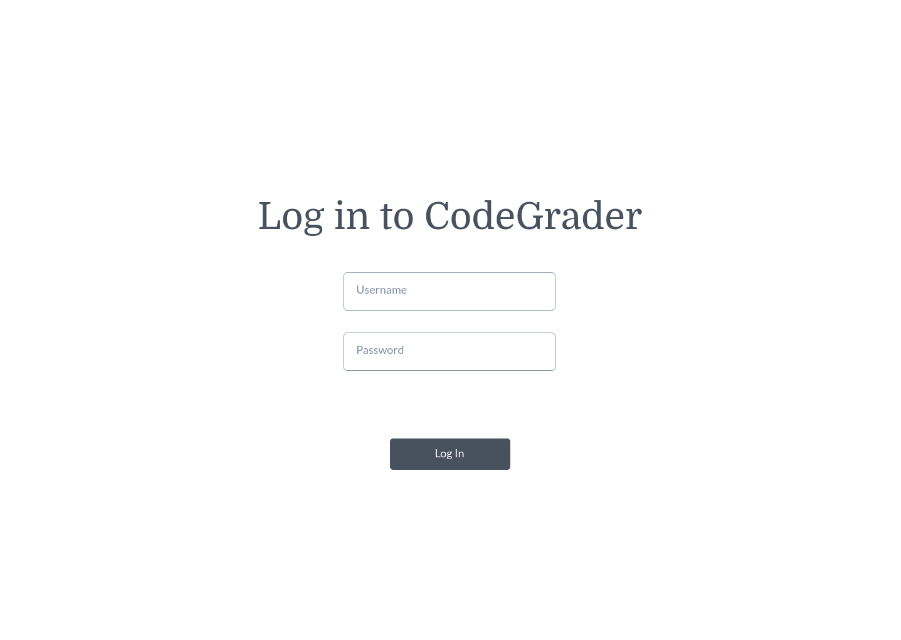
\includegraphics[width=0.8\linewidth]{WireframeLogin.png}

\subsubsection{Instructor Home}
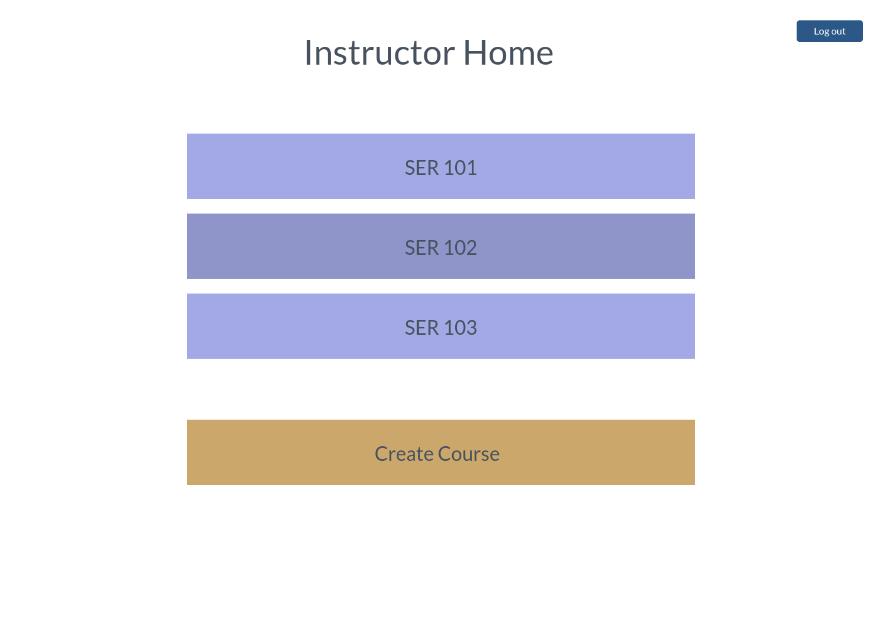
\includegraphics[width=0.8\linewidth]{InstructorHome.png}

\subsubsection{Admin Home}
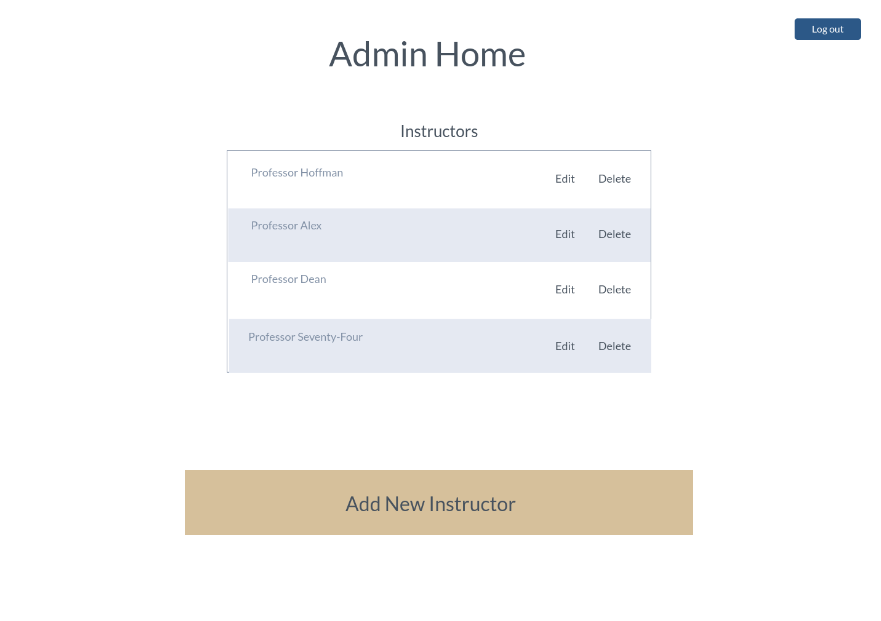
\includegraphics[width=0.8\linewidth]{AdminHome.png}

\subsubsection{Student Home}
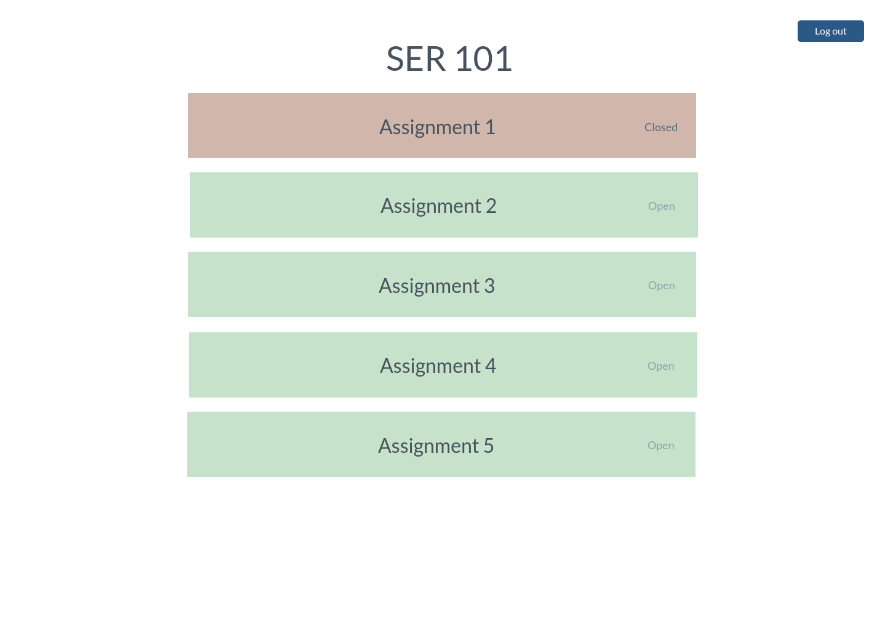
\includegraphics[width=0.8\linewidth]{StudentHome.png}

\subsubsection{Instructor Course View}
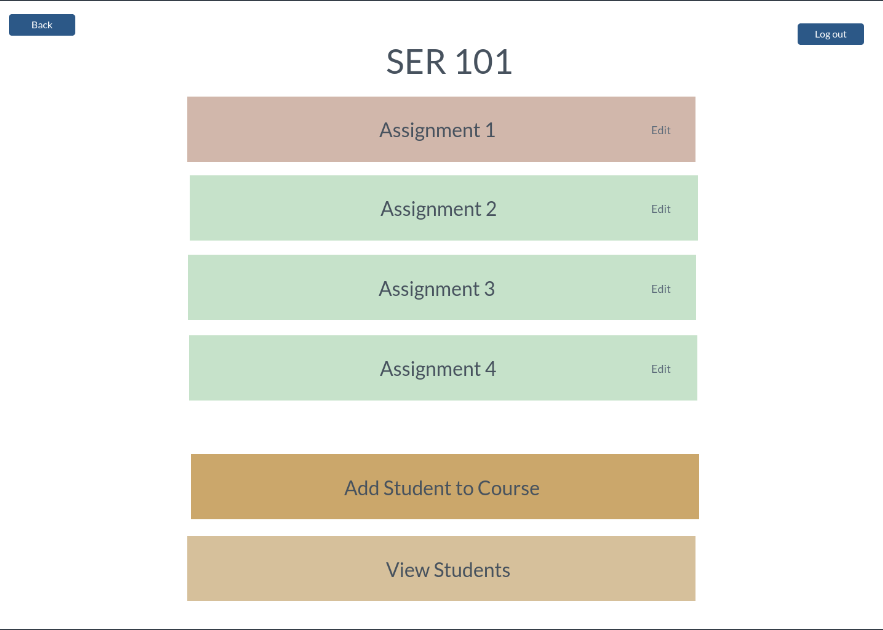
\includegraphics[width=0.8\linewidth]{InstructorCourseView.png}

\subsubsection{Student Grades View}
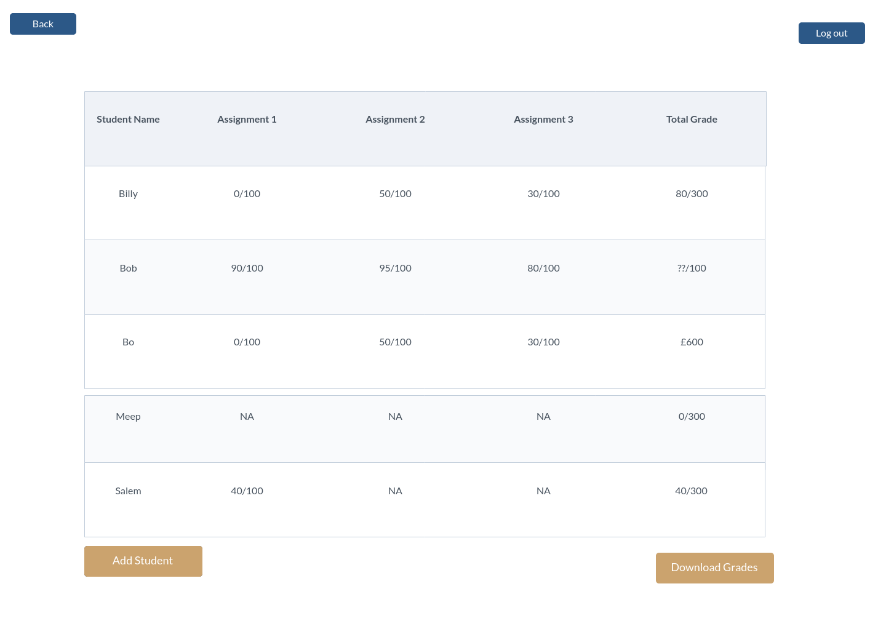
\includegraphics[width=0.8\linewidth]{CourseStudentList.png}

\subsubsection{Create Assignment}
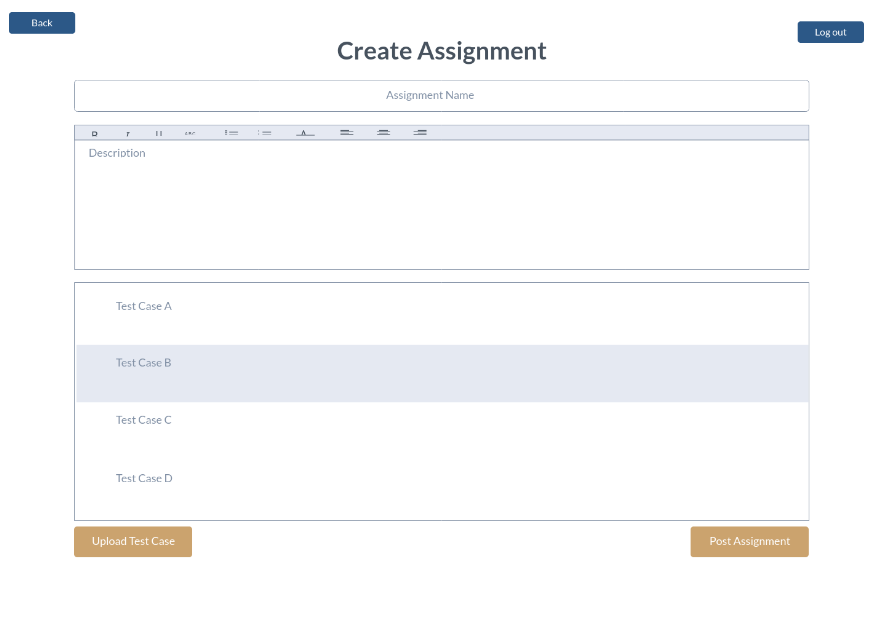
\includegraphics[width=0.8\linewidth]{CreateAssignment.png}

\subsubsection{View Assignment}
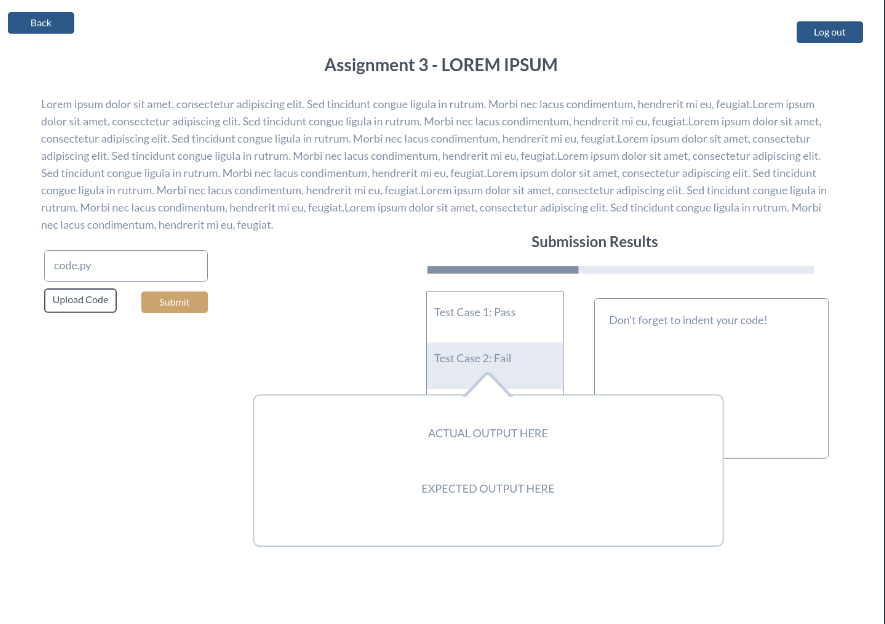
\includegraphics[width=0.8\linewidth]{ViewAssignment.png}

\subsubsection{Instructor View Submission}
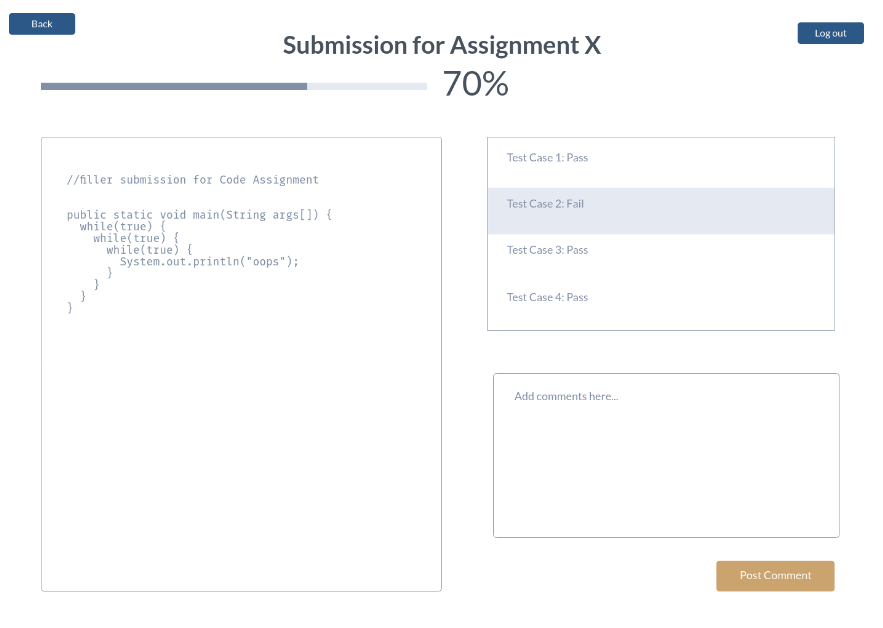
\includegraphics[width=0.8\linewidth]{InstructorViewSubmission.png}

\subsubsection{Create Account}
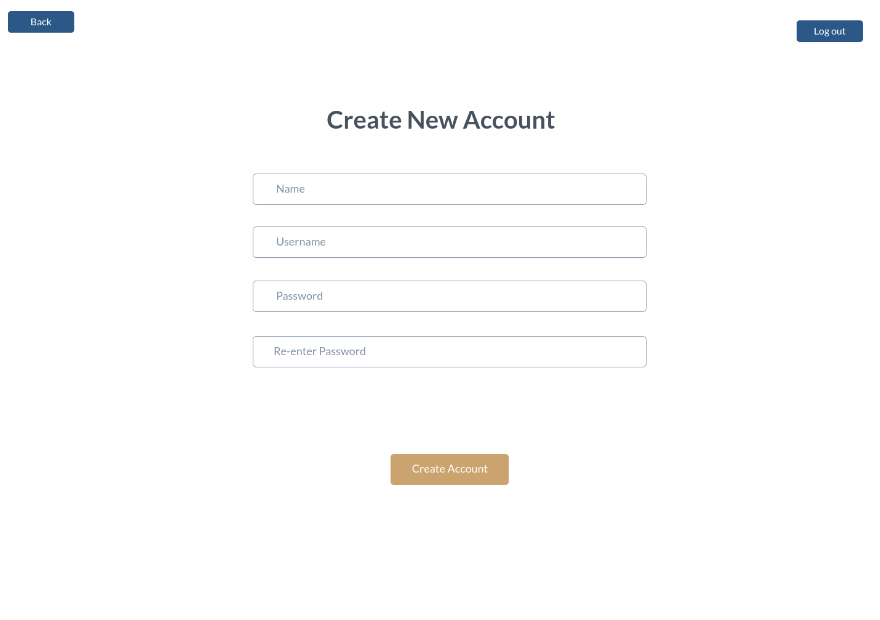
\includegraphics[width=0.8\linewidth]{CreateAccount.png}

\subsubsection{Create Course}
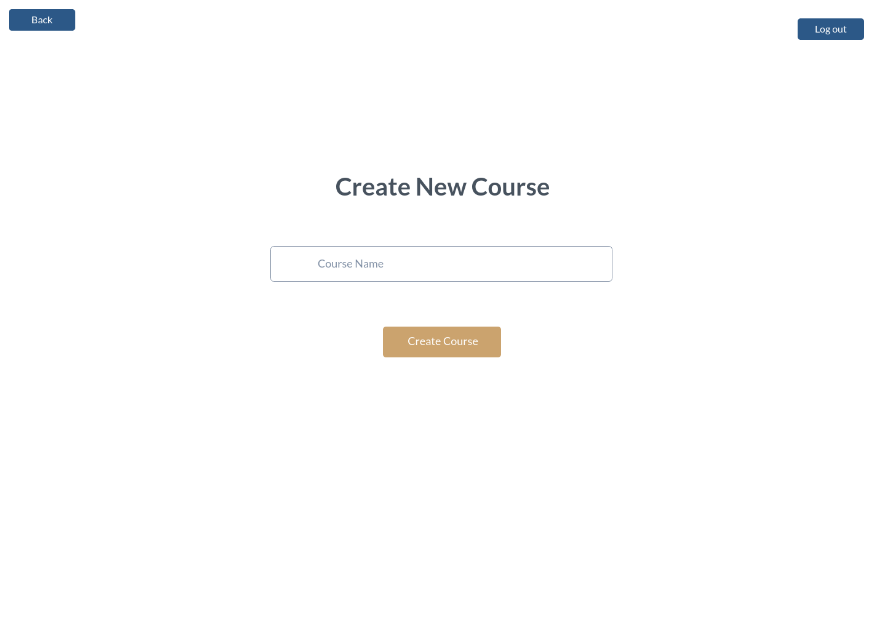
\includegraphics[width=0.8\linewidth]{CreateCourse.png}

\newpage

\subsection{Use Case Diagram}

\includegraphics[height=8in,width=\linewidth,keepaspectratio]{Use Case Diagram.png}

\newpage

\subsection{System Features}

\subsubsection{Login}

\paragraph{Description} An admin, instructor, or student signs into the application using their username and password

\paragraph{Functional Requirements and Use Cases}

\begin{itemize}
  \item \textbf{REQ-1} The system should allow an admin to login using their username and password
  \item \textbf{REQ-2} The system should allow an instructor to login using their username and password
  \item \textbf{REQ-3} The system should allow a student to login using their username and password
\end{itemize}


\vspace{0.1in}

\begin{tabular}{| p{0.25\linewidth} | p{0.65\linewidth} |}
  \hline
  \textbf{Use Case Name} & Login \\
  \hline
  \textbf{Brief Description} & The user logs into their account using their username and password \\
  \hline
  \textbf{Actor(s)} & User \\
  \hline
  \textbf{Pre-conditions} & None\\
  \hline
  \textbf{Basic Flow} & \begin{itemize}
    \item[] \textbf{1} The user opens up the web application
    \item[] \textbf{2} The system prompts the user to sign in using a username and password
    \item[] \textbf{3} The user provides their account's username and password, and submits
    \item[] \textbf{4} The system displays the user's home page
  \end{itemize}\\
  \hline
  \textbf{Alternate Flows} & \begin{itemize}
    \item[] \textbf{3A} The user inputs a username that does not exist
    \item[] \textbf{3A1} The system displays an error stating that either the username or password is incorrect, and asks the user to try signing in again
    \item[] \textbf{3B} The user inputs a password that does not match the user's actual password
    \item[] \textbf{3B1} The system displays an error stating that either the username or password is incorrect, and asks the user to try signing in again
  \end{itemize} \\
  \hline
\end{tabular}

\subsubsection{Create Instructor Account}

\paragraph{Description} An admin creates an instructor account, setting it's username and password


\paragraph{Functional Requirements and Use Cases}

\begin{itemize}
  \item \textbf{REQ-4} The system should allow an admin to create an instructor account with a username and password
\end{itemize}

\vspace{0.1in}

\begin{tabular}{| p{0.25\linewidth} | p{0.65\linewidth} |}
  \hline
  \textbf{Use Case Name} & Create Instructor Account \\
  \hline
  \textbf{Brief Description} & The admin creates an instructor account, and specifies the username and password \\
  \hline
  \textbf{Actor(s)} & Admin \\
  \hline
  \textbf{Pre-conditions} & The admin is logged in, and is on the admin homepage\\
  \hline
  \textbf{Basic Flow} & \begin{itemize}
    \item[] \textbf{1} The admin chooses to create a new instructor account
    \item[] \textbf{2} The system prompts the admin to specify the instructor name, username, and password
    \item[] \textbf{3} The admin fills in the name, username and password, and submits
    \item[] \textbf{4} The system creates the account and returns the admin to the admin homepage
  \end{itemize}\\
  \hline
  \textbf{Alternate Flows} & \begin{itemize}
    \item[] \textbf{3A} The user inputs a username that alraedy exists
    \item[] \textbf{3A1} The system displays an error asking the admin to choose another username
  \end{itemize} \\
  \hline
\end{tabular}

\subsubsection{Create Course}

\paragraph{Description} The instructor creates a course with a name and description


\paragraph{Functional Requirements and Use Cases}
\begin{itemize}
  \item \textbf{REQ-5} The system should allow an instructor to create a new course with a name and description
\end{itemize}

\vspace{0.1in}

\begin{tabular}{| p{0.25\linewidth} | p{0.65\linewidth} |}
  \hline
  \textbf{Use Case Name} & Create Course \\
  \hline
  \textbf{Brief Description} & The instructor creates a course \\
  \hline
  \textbf{Actor(s)} & Instructor \\
  \hline
  \textbf{Pre-conditions} & The instructor is logged in, and is currently on the instructor homepage\\
  \hline
  \textbf{Basic Flow} & \begin{itemize}
    \item[] \textbf{1} The instructor chooses to create a new course
    \item[] \textbf{2} The system prompts the instructor to fill in the new course name
    \item[] \textbf{3} The instructor fills in the details and submits
    \item[] \textbf{4} The system creates the course, and displays the course's page
  \end{itemize}\\
  \hline
  \textbf{Alternate Flows} & \begin{itemize}
    \item[] \textbf{3A} The instructor already has a course with the given coursename
    \item[] \textbf{3A1} The system displays an error asking the instructor to choose another course name
  \end{itemize} \\
  \hline
\end{tabular}

\subsubsection{Create Student Account}

\paragraph{Description} The instructor creates a student accoutn for a course

\paragraph{Functional Requirements and Use Cases}

\begin{itemize}
  \item \textbf{REQ-6} The system should allow an instructor to create a student account for a course with a username and a password
\end{itemize}

\vspace{0.2in}

\begin{tabular}{| p{0.25\linewidth} | p{0.65\linewidth} |}
  \hline
  \textbf{Use Case Name} & Create Student Account \\
  \hline
  \textbf{Brief Description} & The instructor creates a student account for a course \\
  \hline
  \textbf{Actor(s)} & Instructor \\
  \hline
  \textbf{Pre-conditions} & The instructor is logged in, and is at the home page of one of their coruses\\
  \hline
  \textbf{Basic Flow} & \begin{itemize}
    \item[] \textbf{1} The instructor chooses to view the student grades list
    \item[] \textbf{2} The system shows the user a list of all currently enrolled students, and the option to create a new account
    \item[] \textbf{3} The instructor chooses to create a new account
    \item[] \textbf{4} The system prompts the instructor to input the new account's name, username, and password
    \item[] \textbf{5} The user inputs the relevant information and submits
    \item[] \textbf{6} The system creates the user, and then shows an updated list of all students currently enrolled in that course.
  \end{itemize}\\
  \hline
  \textbf{Alternate Flows} & \begin{itemize}
    \item[] \textbf{5A} The instructor inputs a username that already has an account
    \item[] \textbf{5A1} The system asks the instructor to input a different username because the username is currently in use.
  \end{itemize} \\
  \hline
\end{tabular}

\subsubsection{Upload Test Case}

\paragraph{Description} An instructor uploads files required to create a test case for an assignment

\paragraph{Functional Requirements and Use Cases}

\begin{itemize}
  \item \textbf{REQ-7} The system should allow an instructor to upload an input and expected output file as a test case.
\end{itemize}

\vspace{0.2in}
\begin{tabular}{| p{0.25\linewidth} | p{0.65\linewidth} |}
  \hline
  \textbf{Use Case Name} & Upload Test Case \\
  \hline
  \textbf{Brief Description} & The instructor uploads a test case as two files including the input and output \\
  \hline
  \textbf{Actor(s)} & Instructor \\
  \hline
  \textbf{Pre-conditions} & The instructor is logged in, and is currently editing or creating an assignment\\
  \hline
  \textbf{Basic Flow} & \begin{itemize}
    \item[] \textbf{1} The instructor chooses to upload a test case
    \item[] \textbf{2} The system prompts the instructor to upload two documents, one labelled `Input' and the other labelled `Output'
    \item[] \textbf{3} The instructor uploads the input and output files and submits
    \item[] \textbf{4} The system creates the test case, attaches it to the assignment, and returns the instructor to the assignment editor
  \end{itemize}\\
  \hline
  \textbf{Alternate Flows} & \begin{itemize}
    \item[] \textbf{3A} The instructor does not upload an input file
    \item[] \textbf{3A1} The system prints an error and asks the instructor to upload an input file
    \item[] \textbf{3B} The instructor does not upload an output file
    \item[] \textbf{3B1} The system prints and error and asks the instructor to upload an output file
  \end{itemize} \\
  \hline
\end{tabular}

\subsubsection{Create and Update Assignments}

\paragraph{Description} An instructor is able to create and update assignemnts within a course

\paragraph{Functional Requirements and Use Cases}

\begin{itemize}
  \item \textbf{REQ-8} The system allows an instructor to create an assignment with a name, description, and test cases
  \item \textbf{REQ-9} The system allows an instructor to edit any assignment in one of their courses
\end{itemize}

\vspace{0.2in}

\begin{tabular}{| p{0.25\linewidth} | p{0.65\linewidth} |}
  \hline
  \textbf{Use Case Name} & Create Assignment \\
  \hline
  \textbf{Brief Description} & The instructor creates an assignment in one of their couses \\
  \hline
  \textbf{Actor(s)} & Instructor \\
  \hline
  \textbf{Pre-conditions} & The instructor is logged in\\
  \hline
  \textbf{Basic Flow} & \begin{itemize}
    \item[] \textbf{1} The instructor chooses a course
    \item[] \textbf{2} The system displays a list of assignments in that course
    \item[] \textbf{3} The instructor chooses to createan assignment
    \item[] \textbf{4} The system prompts the instructor to input the assignment name, description, and upload any test cases
    \item[] \textbf{5} The instructor inputs the proper data, and submits the assignment
    \item[] \textbf{6} The system displays an updated assignment list with the new assignment
  \end{itemize}\\
  \hline
  \textbf{Alternate Flows} & \begin{itemize}
    \item[] \textbf{3A} The instructor does not upload an input file
    \item[] \textbf{3A1} The system prints an error and asks the instructor to upload an input file
    \item[] \textbf{3B} The instructor does not upload an output file
    \item[] \textbf{3B1} The system prints and error and asks the instructor to upload an output file
  \end{itemize} \\
  \hline
\end{tabular}

\vspace{0.2in}

\begin{tabular}{| p{0.25\linewidth} | p{0.65\linewidth} |}
  \hline
  \textbf{Use Case Name} & Update Assignment \\
  \hline
  \textbf{Brief Description} & The instructor creates an assignment in one of their couses \\
  \hline
  \textbf{Actor(s)} & Instructor \\
  \hline
  \textbf{Pre-conditions} & The instructor is logged in\\
  \hline
  \textbf{Basic Flow} & \begin{itemize}
    \item[] \textbf{1} The instructor chooses a course
    \item[] \textbf{2} The system displays a list of assignments in that course
    \item[] \textbf{3} The instructor chooses to edit one of the assignments in the course
    \item[] \textbf{4} The system displays an editable screen for the assignment, allowing the instructor to edit the name, description, and upload new test cases
    \item[] \textbf{5} The user updates the assignment and submits
    \item[] \textbf{6} The system updates the assignment and displays an updated assignment list
  \end{itemize}\\
  \hline
  \textbf{Alternate Flows} & None \\
  \hline
\end{tabular}

\subsubsection{Submit Assignments}

\paragraph{Description} A student completes and submits an assignemnt for grading

\paragraph{Functional Requirements and Use Cases}

\begin{itemize}
  \item \textbf{REQ-10} The system should allow a student to upload and submit their code for an assignment
\end{itemize}

\vspace{0.2in}

\begin{tabular}{| p{0.25\linewidth} | p{0.65\linewidth} |}
  \hline
  \textbf{Use Case Name} & Submit Assignment \\
  \hline
  \textbf{Brief Description} & The student uploads their code and submits an assignment \\
  \hline
  \textbf{Actor(s)} & Student \\
  \hline
  \textbf{Pre-conditions} & The Student is Logged In\\
  \hline
  \textbf{Basic Flow} & \begin{itemize}
    \item[] \textbf{1} The student chooses an assignment to complete
    \item[] \textbf{2} The system displays details for that assignment, and gives the student the ability to upload code and submit
    \item[] \textbf{3} The student uploads their code and submits
    \item[] \textbf{4} The system uploads the code and submits the assignment
    \item[] \textbf{5} The system grades the assignment, and displays the grading results to the user
  \end{itemize}\\
  \hline
  \textbf{Alternate Flows} & \begin{itemize}
    \item[] \textbf{3A} The student does not upload any file and submits
    \item[] \textbf{3A1} The system prints an error requesting that the user uploads a code file to submit
  \end{itemize}\\
  \hline
\end{tabular}

\subsubsection{View Student Grades}

\paragraph{Description} The instructor views the submission grades of students in a course

\paragraph{Functional Requirements and Use Cases}

\begin{itemize}
  \item\textbf{REQ-11} The system should allow an instructor to view a list of grades in a course
\end{itemize}

\vspace{0.2in}

\begin{tabular}{| p{0.25\linewidth} | p{0.65\linewidth} |}
  \hline
  \textbf{Use Case Name} & View Course Grades \\
  \hline
  \textbf{Brief Description} & The instructor navigates and views a list of course grades \\
  \hline
  \textbf{Actor(s)} & Instructor \\
  \hline
  \textbf{Pre-conditions} & The Instructor is Logged In\\
  \hline
  \textbf{Basic Flow} & \begin{itemize}
    \item[] \textbf{1} The instructor chooses a course
    \item[] \textbf{2} The system displays the list of assignments for the course
    \item[] \textbf{3} The instructor chooses to view course grades
    \item[] \textbf{4} The system displays a table of students and their grades for each assignment
  \end{itemize}\\
  \hline
  \textbf{Alternate Flows} & None\\
  \hline
\end{tabular}

\subsubsection{Download Student Grades}

\paragraph{Description} The instructor downloads student grades as a file

\paragraph{Functional Requirements and Use Cases}

\begin{itemize}
  \item \textbf{REQ-12} The system should allow an instructor to download course grades as a file
\end{itemize}

\vspace{0.2in}

\begin{tabular}{| p{0.25\linewidth} | p{0.65\linewidth} |}
  \hline
  \textbf{Use Case Name} & Download Course Grades \\
  \hline
  \textbf{Brief Description} & The instructor downloads student grades for a particular course \\
  \hline
  \textbf{Actor(s)} & Instructor \\
  \hline
  \textbf{Pre-conditions} & The Instructor is Logged In and is viewing grades for one of their courses\\
  \hline
  \textbf{Basic Flow} & \begin{itemize}
    \item[] \textbf{1} The instructor chooses to download the course grades
    \item[] \textbf{2} The system asks the instructor what file format they want the grades in
    \item[] \textbf{3} The instructor selects a file format
    \item[] \textbf{4} The system compiles the grades into a file of the provided format, and sends it to the instructor
  \end{itemize}\\
  \hline
  \textbf{Alternate Flows} & None\\
  \hline
\end{tabular}

\subsubsection{Provide Submission Feedback}

\paragraph{Description} The instructor provides feedback to the submission of a particular student for a particular assignment

\paragraph{Functional Requirements and Use Cases}

\begin{itemize}
  \item \textbf{REQ-13} The system should allow the instructor to add feedback to a student's assignment submissions
\end{itemize}

\begin{tabular}{| p{0.25\linewidth} | p{0.65\linewidth} |}
  \hline
  \textbf{Use Case Name} & Add Submission Feedback \\
  \hline
  \textbf{Brief Description} & The instructor provides feedback to a submission \\
  \hline
  \textbf{Actor(s)} & Instructor \\
  \hline
  \textbf{Pre-conditions} & The Instructor is Logged In and is currently viewing the list of assignments for a course\\
  \hline
  \textbf{Basic Flow} & \begin{itemize}
    \item[] \textbf{1} The instructor chooses one of the assignment grades for a student
    \item[] \textbf{2} The system displays that submission details, including the submitted code and the test case results. The system also displays an option to add feedback as a comment
    \item[] \textbf{3} The instructor chooses to add feedback
    \item[] \textbf{4} The system prompts the user to input the feedback
    \item[] \textbf{5} The instructor inputs the feedback and submits
    \item[] \textbf{6} The system adds the feedback to the submission and displays the submission
  \end{itemize}\\
  \hline
  \textbf{Alternate Flows} & None\\
  \hline
\end{tabular}

\subsubsection{Delete Instructor Account}

\paragraph{Description} The admin deletes an instructor account

\paragraph{Functional Requirement and Use Cases}

\begin{itemize}
  \item \textbf{REQ-14} The system should allow an admin to delete an instructor account
\end{itemize}

\begin{tabular}{| p{0.25\linewidth} | p{0.65\linewidth} |}
  \hline
  \textbf{Use Case Name} & Delete Instructor Account \\
  \hline
  \textbf{Brief Description} & The admin deletes an instructor account \\
  \hline
  \textbf{Actor(s)} & Admin \\
  \hline
  \textbf{Pre-conditions} & The admin is logged in and sees a list of instructors\\
  \hline
  \textbf{Basic Flow} & \begin{itemize}
    \item[] \textbf{1} The admin chooses to delete an instructor from the list
    \item[] \textbf{2} The system asks the admin if they are sure they would like to delete that account, all courses under that account, and all students in those courses
    \item[] \textbf{3} The admin chooses to confirm and delete the account
    \item[] \textbf{4} The system deletes the account, all courses under the account, and all students under those courses. The system then displays the updated list of instructors to the admin.
  \end{itemize}\\
  \hline
  \textbf{Alternate Flows} & \begin{itemize}
    \item[] \textbf{3A} The admin chooses to cancel
    \item[] \textbf{3A1} The system returns to the admin home page
  \end{itemize}\\
  \hline
\end{tabular}

\subsubsection{Delete Course}

\paragraph{Description} An instructor deletes one of their courses

\paragraph{Functional Requirements and Use Cases}

\begin{itemize}
  \item \textbf{REQ-15} The system should allow the instructor to delete one of their courses
\end{itemize}

\begin{tabular}{| p{0.25\linewidth} | p{0.65\linewidth} |}
  \hline
  \textbf{Use Case Name} & Delete Course\\
  \hline
  \textbf{Brief Description} & An instructor deletes a course\\
  \hline
  \textbf{Actor(s)} & Instructor \\
  \hline
  \textbf{Pre-conditions} & The instructor is currently logged in\\
  \hline
  \textbf{Basic Flow} & \begin{itemize}
    \item[] \textbf{1} The instructor chooses to delete a course from their list of courses
    \item[] \textbf{2} The system asks the instructor if they really wish to delete that course
    \item[] \textbf{3} The instructor confirms they wish to delete the course
    \item[] \textbf{4} The system deletes the course, and all enrolled student accounts
  \end{itemize}\\
  \hline
  \textbf{Alternate Flows} & \begin{itemize}
    \item[] \textbf{3A} The instructor chooses to cancel
    \item[] \textbf{3A1} The system displays an unchanged course list
  \end{itemize}\\
  \hline
\end{tabular}

\subsubsection{Delete Student Account}

\paragraph{Description} An instructor deletes a student account from their course.

\paragraph{Functional Requirements and Use Cases}
\begin{itemize}
  \item \textbf{REQ-16} The system should allow the instructor to delete a student account in one of their courses.
\end{itemize}

\begin{tabular}{| p{0.25\linewidth} | p{0.65\linewidth} |}
  \hline
  \textbf{Use Case Name} & Delete Student Account\\
  \hline
  \textbf{Brief Description} & An instructor deletes a student account from one of their courses\\
  \hline
  \textbf{Actor(s)} & Instructor \\
  \hline
  \textbf{Pre-conditions} & The instructor is currently logged in, and has navigated to the student list in one of their courses\\
  \hline
  \textbf{Basic Flow} & \begin{itemize}
    \item[] \textbf{1} The instructor chooses to delete one of the students
    \item[] \textbf{2} The system asks the instructor if they really wish to delete that student account
    \item[] \textbf{3} The instructor confirms they wish to delete that student account
    \item[] \textbf{4} The system deletes the student account, and updates the student list
  \end{itemize}\\
  \hline
  \textbf{Alternate Flows} & \begin{itemize}
    \item[] \textbf{3A} The instructor chooses to cancel
    \item[] \textbf{3A1} The system displays an unchanged student list
  \end{itemize}\\
  \hline
\end{tabular}

\subsubsection{Edit Instructor Account}

\paragraph{Description} The admin edits the information for an instructor account

\paragraph{Functional Requirement and Use Cases}

\begin{itemize}
  \item \textbf{REQ-17} The system should allow an admin to edit an instructor account's name, username, and password
\end{itemize}

\begin{tabular}{| p{0.25\linewidth} | p{0.65\linewidth} |}
  \hline
  \textbf{Use Case Name} & Edit Instructor Account \\
  \hline
  \textbf{Brief Description} & The admin edits an instructor account \\
  \hline
  \textbf{Actor(s)} & Admin \\
  \hline
  \textbf{Pre-conditions} & The admin is logged in and sees a list of instructors\\
  \hline
  \textbf{Basic Flow} & \begin{itemize}
    \item[] \textbf{1} The admin chooses to edit an instructor account from the list
    \item[] \textbf{2} The system gives the admin the options to change the instructor account's name, username, and password
    \item[] \textbf{3} The admin updates the instructor's information and submits
    \item[] \textbf{4} The system updates the instructor's account and displays an updated list of instructors
  \end{itemize}\\
  \hline
  \textbf{Alternate Flows} & \begin{itemize}
    \item[] \textbf{3A} The admin changes the username to a username that is already in use
    \item[] \textbf{3A1} The system prints an error stating that the username is in use, and asks the admin to choose a new username
  \end{itemize}\\
  \hline
\end{tabular}

\subsubsection{Edit Course}

\paragraph{Description} An instructor edits the information of one of their courses

\paragraph{Functional Requirements and Use Cases}

\begin{itemize}
  \item \textbf{REQ-18} The system should allow the instructor to edit the name of one of their courses
\end{itemize}

\begin{tabular}{| p{0.25\linewidth} | p{0.65\linewidth} |}
  \hline
  \textbf{Use Case Name} & Edit Course\\
  \hline
  \textbf{Brief Description} & An instructor edits a course\\
  \hline
  \textbf{Actor(s)} & Instructor \\
  \hline
  \textbf{Pre-conditions} & The instructor is currently logged in\\
  \hline
  \textbf{Basic Flow} & \begin{itemize}
    \item[] \textbf{1} The instructor chooses to edit a course in their list
    \item[] \textbf{2} The system displays options to change the course name
    \item[] \textbf{3} The instructor updates the course information and submits
    \item[] \textbf{4} The system updates the course information and displays an updated course list
  \end{itemize}\\
  \hline
  \textbf{Alternate Flows} & \begin{itemize}
    \item[] \textbf{3A} The instructor changes the name to a name that is already in use by the instructor
    \item[] \textbf{3A1} The system displays an error saying that the instructor needs to choose a different course name
  \end{itemize}\\
  \hline
\end{tabular}

\subsubsection{Edit Student Account}

\paragraph{Description} An instructor edits a student account in their course.

\paragraph{Functional Requirements and Use Cases}
\begin{itemize}
  \item \textbf{REQ-19} The system should allow the instructor to delete a student account in one of their courses.
\end{itemize}

\begin{tabular}{| p{0.25\linewidth} | p{0.65\linewidth} |}
  \hline
  \textbf{Use Case Name} & Edit Student Account\\
  \hline
  \textbf{Brief Description} & An instructor edits a student account in one of their courses\\
  \hline
  \textbf{Actor(s)} & Instructor \\
  \hline
  \textbf{Pre-conditions} & The instructor is currently logged in, and has navigated to the student list in one of their courses\\
  \hline
  \textbf{Basic Flow} & \begin{itemize}
    \item[] \textbf{1} The instructor chooses to edit one of their students
    \item[] \textbf{2} The system displays options to change the students name, username, and password
    \item[] \textbf{3} The instructor updates the information and submits
    \item[] \textbf{4} The system updates the student account data and displays the updated student list
  \end{itemize}\\
  \hline
  \textbf{Alternate Flows} & \begin{itemize}
    \item[] \textbf{3A} The instructor changes the username to a different username that already exists
    \item[] \textbf{3A1} The system displays an error and asks the instructor to choose a different username
  \end{itemize}\\
  \hline
\end{tabular}

\subsubsection{View Test Case Output}

\paragraph{Description} A student views the output compared to the expected output for a test case in one of their submissions.

\paragraph{Functional Requirements and Use Cases}

\begin{itemize}
  \item \textbf{REQ-20} The system should allow the student to view the actual output compared to the expected output for a test case.
\end{itemize}

\begin{tabular}{| p{0.25\linewidth} | p{0.65\linewidth} |}
  \hline
  \textbf{Use Case Name} & View Test Case Results\\
  \hline
  \textbf{Brief Description} & A student views the test case results for a submission\\
  \hline
  \textbf{Actor(s)} & Student \\
  \hline
  \textbf{Pre-conditions} & The student is signed in, and has submitted an assignment at least once\\
  \hline
  \textbf{Basic Flow} & \begin{itemize}
    \item[] \textbf{1} The student opens an assignment that they have already submitted
    \item[] \textbf{2} The system displays the assignment information, as well as the student's submission. The system displays a list of test cases and whether the student has passed or failed each one
    \item[] \textbf{3} The student chooses one of the test cases
    \item[] \textbf{4} The system displays the details of the test case, including the comparison between the actual result, and expected result
  \end{itemize}\\
  \hline
  \textbf{Alternate Flows} & None\\
  \hline
\end{tabular}

\subsection{Nonfunctional Requirements}

\subsubsection{Performance Requirements}
\begin{itemize}
  \item The system should display a login screen within 2 seconds
  \item The system should grade a submission within 2 minutes
\end{itemize}

\subsubsection{Safety Requirements}
\begin{itemize}
  \item The system should not harm the user under any circumstances
\end{itemize}

\subsubsection{Software Quality Requirements}
\begin{itemize}
  \item The system must hold usernames and passwords in a secure database
  \item Upon login, the system should send a text message or email to authenticate the user
\end{itemize}

\subsubsection{Security Requirements}

\begin{itemize}
  \item To comply with FERPA, the system should restrict student information to only be accessible by either the student or instructor.
\end{itemize}

\newpage
\appendix

\section{Glossary}

\paragraph{Test Case} A test case is an execution instance that tests submission code for expected results. Test cases consist of two parts: an input and output. The input is what is fed into the code, and the output is what the code should output. The actual output is compared with the expected output to pass or fail the test.

\end{document}
